\section{Introdução} \label{chap:introducao}
	%intro geralzona
	O recente espetacular progresso na obtenção e manipulação de informações, em conjunto com o progresso da tecnologia da microeletrônica, comunicação e sensores proporcionou um enorme estímulo no desenvolvimento de sistemas computacionais inteligentes de comunicação além de dispositivos \textit{internet} das coisas (IoT, do inglês \textit{Internet of Things}) e \wearables, todos sendo dispositivos embarcados. %citep{Jozwiak2017}
	%
	O projeto de sistemas computacionais está mais complexo que nunca. A demanda por curto tempo para disponibilidade ao mercado somado ao fato de produtos dever ter propriedades de corretude, rapidez, confiabilidade e preço acessível, representam um desafio para projetistas de sistemas embutidos.
	Sistemas computacionais embarcados (também nomeados pela literatura como sistemas embutidos) possuem muitos componentes implementados tanto em \hs\ e este será o tema principal abordado neste documento.

	% combinação de fpga com cpu
	A tendência popular hoje para \design\ de projeto é a combinação das funções do processador com os recursos dos arranjo de portas programáveis em campo (FPGAs, do inglês \textit{Field-Programmable Gates Array}), formando um sistema computacional híbrido, ou também conhecidos como sistemas configuráveis sobre chip (CSoC, do inglês \textit{Configurable System on a Chip}), exemplo exibido na Figura \ref{fig:i-soc}. %\cite{Plessl2003}
	% Utilização de um processador sintético ou físico
	A unidade de processamento central (CPU, do inglês \textit{Central Processing Unit}) nesses tipos de sistema pode ser implementada em duas formas sendo estas \textit{hard} e \textit{soft} \cores.
	O primeiro é um \core\ dedicado, ou seja, um pedaço de circuito integrado dentro ou não de um FPGA.
	Já o segundo é feito por meio da sintetização e mapeamento de um processador no FPGA com seus recursos lógicos, e assim, o processador é obtido por meio de \design\ e sintetizado na placa por meio das portas lógicas.
	Cada um possui suas vantagens. Ao utilizar um \textit{hard} \core, é possível utilizar todos seus recursos obtendo máxima performance nas atividades executadas, a utilização de um \textit{soft} \core\ permite a extensão da arquitetura \cite{Plessl2003}.

	\begin{figure}[!b] \centering
		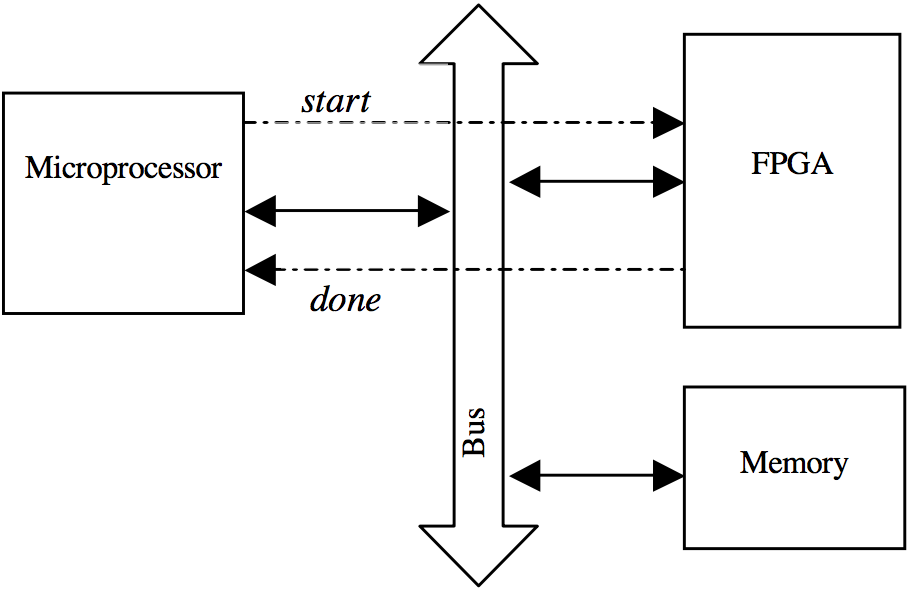
\includegraphics[width=0.35\textwidth]{img/into-soc.png}
		\caption{Visão geral de um CSoC.}
		\label{fig:i-soc}
	\end{figure}

	O conceito de CSoC é importante quando necessita da construção de sistemas computacionais que podem utilizar de circuitos com processadores como é o caso de sistemas embutidos.

	% embedded
    \todo[inline]{A parte de wearable vc tem q explorar mais no capitulo 1 tb, como construcao da motivacao. Uma introducao tem q ser a sequinte sequencia}
	Os sistemas computacionais embutidos são produtos que utilizam processadores e podem estar desde fornos de microondas, até sistemas de controle de aeronaves.
	Requerem técnicas na qual difere das utilizadas para \design\ de computadores de propósito geral ou aplicações de \software\ dessas máquinas \cite{Wolf1994}.
	Em 2015, foi previsto um total de 6,5 bilhões de dispositivos ativamente conectados para o ano de 2016 segundo notícias da empresa de pesquisa e consultoria Gartner \cite{RobvanderMeulen2015}.

	% wearable
	No âmbito de sistemas embutidos, existe um subconjunto na qual possui o propósito de integrar ao sistema corporal expandindo suas capacidades.
	Esses sistemas, chamados de sistemas \wearables, envolvem grande volume de dados de múltiplos sensores complexos ou outros sistemas e são requeridos para prover serviço autônomo contínuo em um longo período de tempo.
	Tais dispositivos demandam de uma alta performance e/ou baixo consumo de energia, sem apresentar \textit{trade-off} de confiabilidade e segurança. %\cite{Jozwiak2017}
	%
	Segundo \cite{Jozwiak2017}, com computação de alta performance e estudos em gasto energético eficiente, foi possível a facilitação do rápido progresso da computação móvel e autônoma.
	Tudo isso deve-se à possibilidade de comunicar-se com a rede global de comunicação, combinada com o progresso de sensores e atuadores, criando novas oportunidades importantes de projeto.
	Exemplos disso são indústrias inteligentes, cidades e casas, bem como setores de \textit{internet} das coisas (IoT, do inglês \textit{Internet of Things}), sistemas móveis como automóveis inteligentes, computação móvel como \textit{smartphones}, comunicação e, não menos importante, os sistemas computacionais \wearable.
	Sendo uma tecnologia pertencente ao conjunto de sistemas embutidos, o sistema computacional \wearable\ pode ser definido como `embutidos que foram inseridos em ambiente \mobile\ de seus usuários, não exercendo a mesma atividade'.
	Um desafio de \design\ para sistemas \wearable\ é combinar a flexibilidade de demanda pelos vários ambientes e aplicações fins de uso e a alta performance exigida em tarefas com o baixo consumo de energia requerido para maximizar o tempo de uso da bateria.


\todo[inline]{1- Apresnetar o problema:}
	% intro particionamento
	A redução do ciclo de comercialização de um produto e o aumento de sua eficiência de desenvolvimento de projeto tem se tornado uma preocupação na área de \design\ de sistemas embarcados, o que inclui os \wearables.
	A técnica de particionamento \hs\ tem sido uma das principais tecnologias para o desenvolvimento de sistemas embarcados desde que, este afeta a performance do sistema como um todo. Para \cite{Hassine2017}, uma das soluções mais elegantes na computação que provê otimizações sistêmicas sobre essas circunstâncias é por meio do particionamento \hs.
	Segundo \cite{Wolf1994}, sistemas embutidos é considerado único pelo fato da necessidade de um \codesign\ de \hs, visando performance, custo e metas de confiabilidade.

	Um exemplo simbólico pode ser ilustrado na Figura \ref{fig:rt-edwards_partitioning} no qual um módulo em \software\ é substituído por um componente em \hardware\ executando a mesma tarefa mas com maior performance.

	\begin{figure}[!b] \centering
		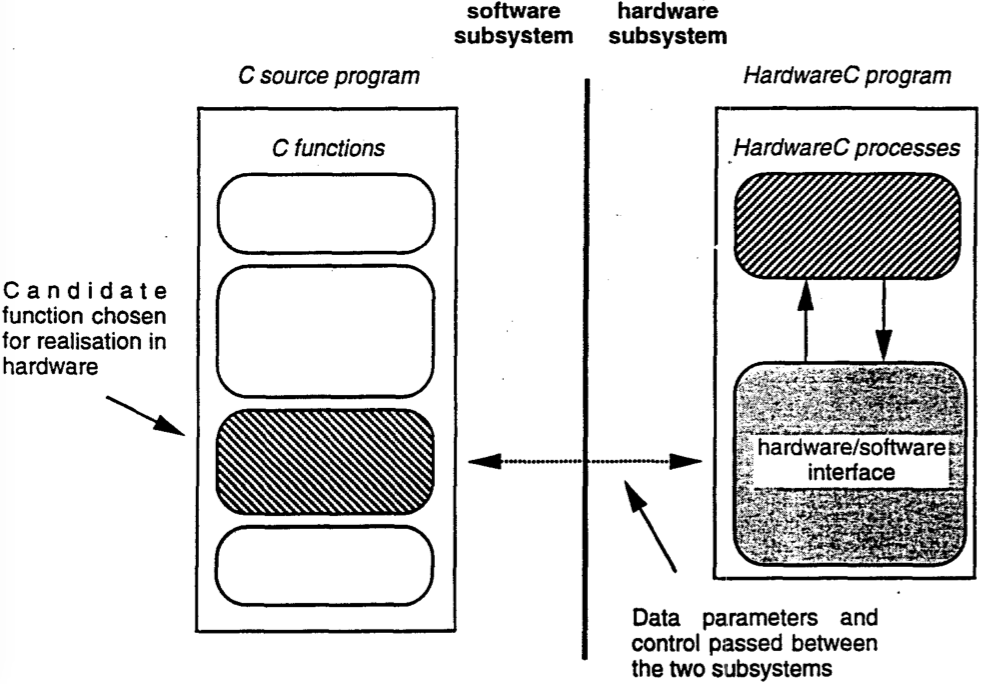
\includegraphics[width=0.37\textwidth]{img/rt-edwards_partitioning.png}
		\caption{Ilustração de um particionamento. Fonte: \cite{Edwards1994}.}
		\label{fig:rt-edwards_partitioning}
	\end{figure}

	\cite{Hidalgo1997} dizem que o objetivo principal do particionamento \hs\ é o balanceamento de todas as tarefas de forma a otimizar alguns objetivos de sistema sobre determinadas restrições.
	A ideia do particionamento é agrupar específicos conjuntos de instruções em uma aplicação e então mapear esses grupos tanto em \hs.
	Os grupos designados ao \software\ são executados sequencialmente pelo respectivo processador do sistema enquanto os mapeados em \hardware\ são implementados por uma combinação customizada ou por circuitos sequenciais \cite{Sass2010}.

	% particionamento
	Quando necessita de performance ao realizar o \codesign\ (termo referente ao inglês \textit{Participatory Design}) de \hs\ para sistemas embutidos, o problema de qual função do sistema deverá ser implementada em \hardware\ ou em \software\ emerge e esse problema é conhecido por particionamento \hs\ (\textit{hardware/software partitioning}).
	Um significante esforço foi posto nesta área nos últimos dez anos, segundo \cite{Trindade2016}.


\todo[inline]{2- Justificativa pq eh um problema relevante:}

	Tradicionalmente, o particionamento é feito manualmente, mas com o desenvolvimento de \designs\ mais complexos em sistemas embarcados, esse problema de decisão torna-se cada vez mais um desafio para os \designers\ de projeto \cite{Trindade2016}.
	Segundo \cite{Edwards1994}, as pesquisas em \codesign\ de \hs\ têm como objetivo o \design\ de sistemas heterogêneos.
	Assim, a meta principal é reduzir o tempo de até a disposição do produto ao mercado bem como a redução do custo dos produtos projetados no qual um projeto de produto normalmente inclui a especificação sistêmica, estimação de custo, o particionamento \hs, a síntese de ambos os projetos e sua simulação \cite{Wolf1994}.

\todo[inline]{3- Motivacao pra resolver este problema:}

	Descrevendo um pouco mais sobre, com o desenvolvimento de complexos \design\ em sistemas embutidos, o particionamento \hs\ tornou-se um problema de otimização em \codesign\ de sistemas \cite{Yan2017}. Tal problema que envolve \design\ colaborativo e multidisciplinar, é um passo chave no \design\ de modernos produtos embutidos \cite{Trappey2016}. Implementações que baseiam-se somente em módulos de \software\ possuem mais flexibilidade e são menos custosas, entretanto, seu custo eleva-se em termos de tempo de execução, o que já não acontece no mundo de \design\ de projetos em \hardware\ \cite{Zhang2008, Hassine2017, Wolf1994}.

	Como o grande requisito para eficiência necessariamente segue junto com a alta velocidade de processamento, existem vários métodos que abordam o problema de particionamento \cite{Arato2005} desde métodos manuais quanto a utilização de meta-heurísticas.

	Dessa forma, ao utilizar o FPGA para o problema de particionamento, é possível acelerar uma aplicação em \hardware\ na qual pode fornecer uma ordem de magnitude de melhoria no desempenho e eficiência de energia em comparação com o \software\ que está sendo executado inteiramente em um processador \cite{Cong2009, Lo2009, Zhang2008a}. Um exemplo de sucesso é o anúncio da Microsoft em \cite{Putnam2014} na qual aceleraram o \textit{Bing Search} em duas vezes com a utilização de FPGAs em seus \textit{data centers} \cite{Putnam2014} além da aquisição da Altera, uma das duas maiores vendedoras de FPGAS no mundo, pela Intel em \cite{Maan2015} por cerca de $ 16.7 $ bilhões de dólares \cite{Maan2015}.


\todo[inline]{4- Contribuicao ao resolver o problema:}


\todo[inline]{5- Objetivos:}

\subsection{Objetivos da Dissertação}
	Este trabalho tem como objetivo a apresentação do problema de particionamento \hs\ bem como sua importância no mundo de sistemas computacionais embutidos, com foco em sistemas \wearables\ apresentando algumas soluções utilizadas atualmente \todo{e a solução proposta}.

    \begin{itemize}
    	\item Introduzir o projeto de sistemas computacionais \wearable;
        \item Apresentação da abordagem metodológica para o uso da solução do problema ao aplicado no contexto desses sistemas.
    \end{itemize}


\subsection{Organização da Dissertação}
	Os demais capítulos deste trabalho estão organizados da seguinte forma: No Capítulo \ref{chap:revisao_bibliografica} é apresentada uma revisão bibliográfica do problema, abordando alguns métodos de fundamental importância para este trabalho. No Capítulo \ref{chap:relacionados} são descritos alguns trabalhos relacionados ao tema abordado. No Capítulo \ref{chap:desenvolvimento} são apresentadas as metodologias. No Capítulo \ref{chap:experimentos} \todo{são?} apresentados os resultados e suas considerações para o problema. No Capítulo \ref{chap:conclusao} são apresentadas as conclusões finais e propostas de trabalhos futuros.
